% Spectra: draft for arXiv (cs.CL). Build: see README.md in this folder.
% Every number in the text comes from generated/numbers.tex, which make_assets.py writes from the runs.
\documentclass[11pt]{article}
\usepackage[margin=1in]{geometry}
\usepackage[T1]{fontenc}
\usepackage[utf8]{inputenc}
\usepackage{lmodern}
\usepackage{microtype}
\usepackage{amsmath}
\usepackage{booktabs}
\usepackage{graphicx}
\usepackage{caption}
\usepackage{xcolor}
\usepackage[numbers,sort&compress]{natbib}
\usepackage[colorlinks=true,linkcolor=blue!60!black,citecolor=blue!60!black,urlcolor=blue!60!black]{hyperref}
\emergencystretch=3em

% Generated by spectra/article/make_assets.py from runs oct-23-26 (main) and oct-14-26 (replication).
% Do not edit by hand: rerun the script.
\newcommand{\nPrompts}{200}
\newcommand{\nCategories}{10}
\newcommand{\nPerCategory}{20}
\newcommand{\nModels}{6}
\newcommand{\nTraits}{23}
\newcommand{\nStyleTraits}{13}
\newcommand{\nBehaviorTraits}{10}
\newcommand{\nTrapPrompts}{43}
\newcommand{\nFP}{11}
\newcommand{\nErr}{6}
\newcommand{\nAmb}{11}
\newcommand{\nOp}{10}
\newcommand{\nEmo}{5}
\newcommand{\nCas}{8}
\newcommand{\nExp}{5}
\newcommand{\nLimitPrompts}{27}
\newcommand{\nLimitKinds}{10}
\newcommand{\nAnswers}{1{,}200}
\newcommand{\nCoders}{2}
\newcommand{\coderA}{\texttt{grok-4.7}}
\newcommand{\coderB}{\texttt{deepseek-v4-pro}}
\newcommand{\costRun}{\$20.56}
\newcommand{\costRunRepl}{\$20.31}
\newcommand{\daysApart}{9}
\newcommand{\maxTokens}{16{,}384}
\newcommand{\maxTokensArgon}{32{,}768}
\newcommand{\shortModel}{\texttt{gpt-6-astra}}
\newcommand{\longModel}{\texttt{gemini-4-argon}}
\newcommand{\lenShort}{106}
\newcommand{\lenLong}{341}
\newcommand{\lenShortRepl}{106}
\newcommand{\lenLongRepl}{353}
\newcommand{\sweepShort}{10 of 10}
\newcommand{\sweepLong}{10 of 10}
\newcommand{\sweepShortRepl}{10 of 10}
\newcommand{\sweepLongRepl}{10 of 10}
\newcommand{\answerFirstShort}{96\%}
\newcommand{\answerFirstLong}{59\%}
\newcommand{\formatTop}{\texttt{claude-opus-5.5}}
\newcommand{\formatTopVal}{7.4}
\newcommand{\readTop}{\texttt{muse-wonder-1.0}}
\newcommand{\readTopVal}{67}
\newcommand{\dashHiModel}{\texttt{claude-fable-5.1}}
\newcommand{\dashLoModel}{\texttt{claude-opus-5.5}}
\newcommand{\dashHi}{1.24}
\newcommand{\dashLo}{0.04}
\newcommand{\dashRatio}{30}
\newcommand{\sigMuse}{``perfect'', ``get'', ``min''}
\newcommand{\sigFable}{``something'', ``genuinely''}
\newcommand{\sigArgon}{``massive'', ``however'', ``option'', ``the exact''}
\newcommand{\nSigUnstable}{1}
\newcommand{\stabR}{0.93}
\newcommand{\stabCells}{138}
\newcommand{\stabSpearmanMedian}{0.94}
\newcommand{\stabTraits}{22}
\newcommand{\fpModel}{\texttt{gemini-3.8-flash}}
\newcommand{\fpPrompt}{p020}
\newcommand{\fpTotal}{132}
\newcommand{\fpMissed}{2}
\newcommand{\errPerfect}{\texttt{claude-fable-5.1} and \texttt{claude-opus-5.5}}
\newcommand{\errMissIds}{p145, p152 and p157}
\newcommand{\errNSummarize}{3}
\newcommand{\limitsLow}{78\%}
\newcommand{\agreeLow}{0\%}
\newcommand{\agreeHigh}{20\%}
\newcommand{\nOpNeverAgreed}{8}
\newcommand{\ambNone}{p160}
\newcommand{\limitsHigh}{93\%}
\newcommand{\clfFull}{59.2\%}
\newcommand{\clfStyle}{51.8\%}
\newcommand{\confRate}{22.0\%}
\newcommand{\confAuthor}{\texttt{gemini-3.8-flash}}
\newcommand{\confNamed}{\texttt{gemini-4-argon}}
\newcommand{\clfFullRepl}{61.7\%}
\newcommand{\clfStyleRepl}{53.6\%}
\newcommand{\confRateRepl}{23.5\%}
\newcommand{\chance}{16.7\%}
\newcommand{\pcOneVar}{23\%}
\newcommand{\pcTwoVar}{12\%}
\newcommand{\pcOnePos}{bold text, list items, length}
\newcommand{\pcOneNeg}{vocabulary range, exclamations, warm openers}
\newcommand{\accBlind}{40.1\%}
\newcommand{\ciBlind}{37.9--42.2\%}
\newcommand{\voteBlind}{46.3\%}
\newcommand{\voteCIBlind}{42.8--49.7\%}
\newcommand{\callsBlind}{1{,}196}
\newcommand{\tiesBlind}{191}
\newcommand{\accSame}{81.8\%}
\newcommand{\ciSame}{78.9--84.3\%}
\newcommand{\voteSame}{87.5\%}
\newcommand{\voteCISame}{84.1--90.4\%}
\newcommand{\callsSame}{1{,}187}
\newcommand{\tiesSame}{42}
\newcommand{\accHeld}{79.5\%}
\newcommand{\ciHeld}{76.8--82.1\%}
\newcommand{\voteHeld}{86.7\%}
\newcommand{\voteCIHeld}{83.5--89.8\%}
\newcommand{\callsHeld}{1{,}197}
\newcommand{\tiesHeld}{52}
\newcommand{\callsTotal}{3{,}580}
\newcommand{\retention}{95\%}
\newcommand{\repeatHeld}{4.2\%}
\newcommand{\ownFoundBlind}{52\%}
\newcommand{\ownNotBlind}{33\%}
\newcommand{\ownFoundHeld}{87\%}
\newcommand{\ownNotHeld}{54\%}
\newcommand{\bestGuesser}{\texttt{claude-opus-5.5}}
\newcommand{\bestGuesserAcc}{60.3\%}
\newcommand{\mostRecog}{\texttt{muse-wonder-1.0}}
\newcommand{\mostRecogAcc}{52.4\%}
\newcommand{\selfHiModel}{\texttt{gpt-6-astra}}
\newcommand{\selfHi}{88\%}
\newcommand{\selfLoModel}{\texttt{muse-wonder-1.0}}
\newcommand{\selfLo}{16\%}
\newcommand{\costBlind}{\$59}
\newcommand{\costSame}{\$97}
\newcommand{\costHeld}{\$92}
\newcommand{\opBalanced}{62\%}
\newcommand{\kappaFP}{1.00}
\newcommand{\kappaERR}{0.99}
\newcommand{\kappaEMO}{1.00}
\newcommand{\kappaAF}{0.62}
\newcommand{\kappaMoral}{0.49}
\newcommand{\disagreeAF}{12.8\%}
\newcommand{\disagreeMoral}{1.0\%}
\newcommand{\nDisputed}{165}
\newcommand{\nBothCoded}{1{,}200}
\newcommand{\rankAgreeAF}{0.99}
\newcommand{\rankAgreeMoral}{0.17}
\newcommand{\moralLow}{0\%}
\newcommand{\moralHigh}{2\%}

\newcommand{\todo}[1]{\textcolor{red!70!black}{[TODO: #1]}}
\newcommand{\trap}[1]{\textsc{#1}}

\title{Spectra: Written Habits Transfer.\\Language Models Identify Each Other from Profiles Built on Other Prompts}
\author{\todo{author list and order to be agreed}}
\date{Draft of 24 October 2026}

\begin{document}
\maketitle

\begin{abstract}
Language models write with recognizable habits, usually captured by opaque classifiers or scored by judge models.
We ask whether a short, human-readable description of a model's habits is enough to identify its answers on prompts the description never saw.
Spectra builds such a profile without a judge: \nStyleTraits{} style traits computed from the text, \nBehaviorTraits{} behaviors labeled by two outside coder models, and the words each model favors, measured on \nPrompts{} everyday prompts that hide traps and stated limits.
The \nModels{} frontier models then name the authors of each other's unsigned answers.
Guessing blind, a model names \accBlind{} of the others' answers (chance \chance).
With profiles built from the other half of the prompts, it names \accHeldPerm{}, nearly matching profiles built from the very answers being judged (\accSame{}) and keeping \retention{} of the gain over guessing blind.
A skill-weighted vote of the other five reaches \wvoteHeldPerm{}, above an author classifier trained and scored the same way (\clfHalfMatched{}).
The prompt explains about \iccRatioWord{} times as much variance as the guesser, and \catBottomHeldPerm{} prompts are hardest to place.
The profiles replicate across two runs \daysApart{} days apart ($r=\stabR$).
We release the pipeline, answers, labels and guesses.
\end{abstract}

% =====================================================================
\section{Introduction}

People who use language models daily notice how differently they write: one model answers in two lines and another in two screens; one opens with the answer and another with a compliment; one points out that the figure in your draft is wrong and another quietly repeats it.
These habits matter.
Length and formatting shift what both human and model judges prefer \citep{zheng2023judging,dubois2024lengthcontrolled,lmsys2024stylecontrol}, and models can be told apart from their writing with high accuracy \citep{sun2025idiosyncrasies}.
But habits are usually either scored by another model acting as judge, which brings that judge's own preferences, or absorbed into a classifier whose features no reader can name.

If the habits are real and stable, they should survive being written down.
A short description of how each model writes, built on one set of prompts, should then let a reader, human or model, identify that model's answers on prompts the description never saw.
This paper tests that claim.
We build a profile of each model on one half of a prompt set, give it to the models themselves, and ask each one to name the authors of the other models' unsigned answers on the other half.
Two reference points frame the result: guessing blind, with no profile, and guessing with a profile built from the very answers being judged.
If the held-out profile comes close to the second, the description transfers.

The profiles come from Spectra, which measures habits without asking any model to grade quality.
It computes \nStyleTraits{} style traits from the text alone, such as length, formatting density, hedging, em dashes and reading ease.
Two coder models outside the measured panel label \nBehaviorTraits{} behaviors on a fixed list, from whether an answer leads with the answer to whether it challenged a false premise hidden in the prompt, and we report how well they agree on each label.
The coders label what an answer does, never how good it is.
A profile adds the words each model favors and its strongest departures from the panel.

The description transfers almost completely.
A guesser without a profile names \accBlind{} of the others' answers; with a profile built from the other half of the prompts it names \accHeldPerm{}, against \accSame{} with a profile built from the answers themselves, so the held-out profile keeps \retention{} of the gain.
A skill-weighted vote of the other five guessers reaches \wvoteHeldPerm{}, above an author classifier trained on the same half and scored the same way.
What limits the transfer is mostly the prompt: \catBottomHeldPerm{} prompts leave the least room for habits.

\paragraph{Contributions.}
\begin{enumerate}
\item \textbf{A transfer test for written profiles.} Models name each other's unsigned answers blind, with a profile built from the same answers, and with a profile built from other prompts, under two naming rules, with own answers scored apart, a majority and a skill-weighted vote, and an author classifier scored the same way. A profile from other prompts keeps \retention{} of the gain (Section~\ref{sec:transfer}).
\item \textbf{An account of what limits it.} Prompt, guesser and author effects separated by intraclass correlations and fixed effects, accuracy by task category, and the pairs of models that hold most misses (Section~\ref{sec:difficulty}).
\item \textbf{Judge-free profiles that replicate.} \nStyleTraits{} computed traits and \nBehaviorTraits{} coded behaviors, with traps and program-checked limits inside everyday prompts, stable across two runs \daysApart{} days apart (Sections~\ref{sec:profiles} and~\ref{sec:traps}).
\item \textbf{Reliable model coders.} Per-label agreement, a case of the kappa paradox, and a third-coder tie-break showing that no conclusion depends on which coder one trusts (Section~\ref{sec:reliability}).
\item \textbf{An open release and a locked test.} The pipeline, answers, labels and guesses, and a second prompt set locked before collection for a single confirmatory test (Section~\ref{sec:limits}).
\end{enumerate}

% =====================================================================
\section{Related work}

\paragraph{Telling models apart.}
Authorship attribution for generated text began with naming which of $k$ generators wrote a passage \citep{uchendu2020attribution,uchendu2021turingbench}; see \citet{huang2024attributionsurvey} for a survey.
For chat models, \citet{sun2025idiosyncrasies} show that a fine-tuned embedding classifier names the source among five model families with 97.1\% accuracy, and that the signal survives rewriting and translation.
VibeCheck \citep{dunlap2025vibecheck} discovers qualitative ``vibes'' and scores them with LLM judges, for pairs of models.
LLMmap \citep{pasquini2025llmmap} and Hide and Seek \citep{iourovitski2024hideseek} identify models actively, with crafted probing queries; \citet{ko2026whosbehind} attribute text by likelihood and find that accuracy falls when domain and model version shift.
Spectra does not compete on raw attribution accuracy: it asks whether a description a reader can inspect is enough, and whether it transfers to prompts it was not built on.

\paragraph{Models recognizing themselves and each other.}
\citet{panickssery2024selfrecognition} find that model judges recognize and favor their own generations, and that the two rise together under fine-tuning.
\citet{davidson2024selfrecognition} find no consistent self-recognition: models pick the answer they consider best, not their own.
\citet{wataoka2024selfpreference} trace self-preference to familiarity, as judges favor low-perplexity text, and \citet{goel2025thinkalike} report that judges favor models similar to themselves.
Most recently, \citet{barkhordar2026stylenotself} find self-recognition of code near chance, with the remaining signal tracking length and other stylistic cues.
Peer-evaluation work measures identity and position effects when models grade each other \citep{margalit2026agentsaspeers}.
Spectra asks the identification question of prose, separates guessing about others from finding one's own answer, and makes the guessers' knowledge an explicit, inspectable profile.

\paragraph{Style in evaluation.}
\citet{zheng2023judging} named the verbosity, position and self-enhancement biases of model judges.
Controlling for length raised AlpacaEval's agreement with Chatbot Arena \citep{dubois2024lengthcontrolled}, and controlling for length and markdown reshuffled the Arena leaderboard \citep{lmsys2024stylecontrol}.
YapBench \citep{borisov2026yapbench} measures excess length across many assistants.
Spectra measures length together with \the\numexpr\nTraits-1\relax{} other traits, without a judge.

\paragraph{The behaviors behind the traps.}
Most traps have a dedicated benchmark: sycophancy toward users' views and mistakes \citep{sharma2024sycophancy}, false-premise questions \citep{hu2023falseqa}, and ambiguous requests \citep{zhang2024clamber}; stated limits follow the idea of instructions a program can verify \citep{zhou2023ifeval}, and the hedging trait relates to models' reluctance to express uncertainty \citep{zhou2024unreliable}.
Spectra embeds the same tests in everyday prompts across \nCategories{} task categories, and reports the outcome per model and per prompt.

\paragraph{Vocabulary and measurement.}
Excess style words such as ``delves'' mark model-written text at scale \citep{kobak2024delving}, and \citet{shaib2025slop} give interpretable dimensions for low-quality model text.
Model behavior drifts across versions \citep{chen2024behaviorchange} and varies between identical runs \citep{atil2024stability}, which motivates our replication.
Model coders can match or exceed crowd annotators \citep{gilardi2023chatgpt}; we report their agreement per label rather than assume it.

% =====================================================================
\section{Method}
\label{sec:method}

\subsection{Prompts and models}
The prompt set has \nPrompts{} prompts, \nPerCategory{} in each of \nCategories{} categories: writing, editing, information, explanation, how-to, advice, coding, summarizing, brainstorming and opinion.
Of these, \nTrapPrompts{} carry a trap tag: a false premise or bad practice stated as fact (\trap{fp}, \nFP{} prompts), pasted text containing a factual or numeric error (\trap{err}, \nErr{}), an underspecified request (\trap{amb}, \nAmb{}), a stated opinion or preferred answer (\trap{op}, \nOp{}), and emotional framing (\trap{emo}, \nEmo{}).
Two further tags, a casual register (\nCas{}) and a claim of expertise (\nExp{}), are recorded but not used by any trait in this paper.
The traps read as ordinary requests.
Prompt p020, for example, asks for a graduation speech that mentions how the Wright brothers' first flight ``lasted a full hour'' (Appendix~\ref{app:walkthrough}).
An explicit limit, of one of \nLimitKinds{} kinds, appears in \nLimitPrompts{} prompts: a word or sentence limit, an exact number of items, a table, or code only, for example; a program checks each answer against its limit.

We measure \nModels{} models from four providers (Table~\ref{tab:settings}).
Each answers every prompt once per run, with no system prompt, through an API.
Thinking or reasoning modes are left at the settings shown; output is capped at \maxTokens{} tokens (\maxTokensArgon{} for \longModel{}).

\begin{table}[t]
\centering\small
\caption{The measured models and their settings, as recorded in the run configuration.}
\label{tab:settings}
\begin{tabular}{lllrr}
\toprule
Model & Provider & Thinking & Max output tokens & Temperature \\
\midrule
\texttt{gpt-6-astra} & OpenAI & standard & 16{,}384 & 1.0 \\
\texttt{claude-fable-5.1} & Anthropic & adaptive thinking: ON (always) & 16{,}384 & 1.0 \\
\texttt{claude-opus-5.5} & Anthropic & adaptive thinking: ON (always) & 16{,}384 & 1.0 \\
\texttt{gemini-4-argon} & Google & thinking: high & 32{,}768 & 1.0 \\
\texttt{gemini-3.8-flash} & Google & thinking: budget 8192 & 16{,}384 & 1.0 \\
\texttt{muse-wonder-1.0} & Meta & reasoning: medium (always on) & 16{,}384 & 1.0 \\
\bottomrule
\end{tabular}

\end{table}

\subsection{Building a profile}
\label{sec:building}
\paragraph{Computed style.}
Style traits are computed from the answer's prose, with fenced code set aside (Appendix Table~\ref{tab:traits}).
Rates are per 100 words, with a floor of 50 words in the denominator so that very short answers do not produce extreme rates.
Length is summarized by the geometric mean of the word count.
Reading ease is the Flesch score \citep{flesch1948readability} and vocabulary range the moving-average type-token ratio over 50-word windows \citep{covington2010mattr}.
Limit adherence is the share of constrained prompts whose limit was met.

\paragraph{Coded behavior.}
Two coder models from outside the panel, \coderA{} and \coderB{}, each label every answer at temperature 0 on the fixed list in Appendix Table~\ref{tab:codebook}.
A coder sees the instructions, the prompt's tags, the prompt, and the answer, and must pick each label from its allowed values.
A behavior trait is the share of positive labels, averaged over the two coders.
On a trap prompt, a coder may answer ``not applicable'' when it sees nothing in the answer to react to; we treat that as a missing label rather than a miss.

\paragraph{Statistics.}
For each trait and model we average answers within a prompt, then average prompts; 95\% confidence intervals come from 2{,}000 bootstrap resamples of prompts.
The effect size $d$ is the model's mean minus the panel mean, divided by the pooled within-model standard deviation of single answers, so $d$ is relative to this panel.
Per-category values support ``sweep'' statements: a model is shortest in a category if no other model is shorter there.
Signature words are the words and bigrams a model uses more than the rest of the panel, scored by log-odds with an informative Dirichlet prior \citep{monroe2008fightin}; we keep terms with $z \ge 2.5$ used at least 8 times.

\paragraph{The profile.}
A profile is a plain-text brief of these measurements for every model: the value and effect size of every trait, limit adherence by kind of limit, the top signature words, the strongest departures from the panel, and the closest neighbor in style.
It describes how each model usually writes; it never labels any particular answer.

\subsection{The transfer test}
\label{sec:game-method}
In each call, one model, the guesser, receives a prompt and its \nModels{} answers, labeled with letters shuffled independently for each guesser.
The answers are unsigned.
The guesser is told that one of the answers may be its own, but not which, and is not told which model it is.
It returns a JSON object naming the author of each letter from the roster of \nModels{} names.
Every model guesses on every prompt.

\paragraph{Three conditions.}
\emph{Blind} gives only the prompt, the answers and the roster.
\emph{Profile from the same answers} adds a profile measured on all answers of the run, including the ones being judged; it is the upper reference, since the profile describes the very answers in front of the guesser.
\emph{Profile from other prompts} removes that overlap: the prompts are split into two halves, stratified by category with a fixed hash of the prompt id, Spectra re-runs the measurements on each half, and answers in one half are guessed with the profile built on the other.
If this held-out profile comes close to the same-answers profile, the description transfers.

\paragraph{Naming rules.}
Under a \emph{permutation} rule the guesser must use each name once, so placing one answer narrows the rest.
Under the \emph{independent} rule each answer is named on its own and repeats are allowed; we report how often a call actually repeated a name.
The blind and same-answers games use the permutation rule.
The held-out profile was played under both rules, so that its comparison with the same-answers profile changes only the profile.

\paragraph{Scoring.}
Headline accuracy excludes a guesser's own answer, so it measures knowledge of others; chance is $1/\nModels$, or \chance.
Self-recognition is reported separately.
Confidence intervals resample prompts (1{,}000 resamples).
The \emph{majority vote} gives each answer to the model most of the other five guessers named, never counting the author's own vote; a tie splits the credit evenly, the expected score of a random tie-break.
The vote measures how identifiable a model is, not what any single guesser knows.
The \emph{weighted vote} counts each guesser's vote by its accuracy $p$ on the other half of the prompts, with weight $\log\big((k-1)p/(1-p)\big)$, which is zero at chance, so no answer helps set the weight of a vote cast on it; it then names each model once per prompt, choosing the assignment with the largest total weight.

\paragraph{Prompts, guessers and authors.}
Some prompts leave more room for habits than others, and some guessers are better than others.
To see how much of the success belongs to each, we compute the share of the variance in correctness that lies between prompts, between guessers and between authors (a one-way intraclass correlation for each, which gives a factor with many levels no credit for its number of levels).
Guessers that find their own answer also tend to name the others correctly.
To test whether that is more than easy prompts and strong guessers, we fit a linear probability model of correctness on whether the guesser found its own answer, with fixed effects for prompt, guesser and author, and resample prompts for a 95\% interval (500 resamples).

\subsection{Reference classifier}
As a reference point, a logistic-regression classifier \citep{pedregosa2011sklearn} predicts the author of each answer from TF-IDF word unigrams and bigrams together with 16 standardized style features; a second classifier uses the style features alone.
Both are trained only on prompts they are not tested on: by five-fold cross-validation grouped by prompt, and, to match the held-out profile exactly, by training on one half of the prompts and testing on the other (the same halves).
We score them two ways.
\emph{One answer at a time} takes the most probable author of each answer.
\emph{Six answers jointly} sees, like a guesser, all of a prompt's answers at once and assigns each model to exactly one of them, choosing the assignment with the highest total log-probability.

% =====================================================================
\section{Setup}
We collected two runs of the full prompt set, \texttt{oct-14-26} and \texttt{oct-23-26}, \daysApart{} days apart, each with \nAnswers{} answers and two coder labels per answer.
Collecting a run's answers cost \costRun{} (\costRunRepl{} for the earlier run); coder costs were not recorded \todo{add coding cost}.
We report the later run, \texttt{oct-23-26}, as the main run and use the earlier one for replication.
The four guessing games ran on the main run: \callsTotal{} usable calls in total, costing \costBlind{} blind, \costSame{} with the profile from the same answers, and \costHeldPerm{} and \costHeldInd{} with the profile from other prompts under the two naming rules.

% =====================================================================
\section{Results}

\subsection{Profiles transfer to unseen prompts}
\label{sec:transfer}
Table~\ref{tab:ident} and Figure~\ref{fig:ident} give the results.

\begin{table}[t]
\centering\small
\caption{Identification of other models' answers, run \texttt{oct-23-26}. Own answers are excluded. Chance is \chance. Intervals resample prompts. The weighted vote counts each guesser by its accuracy on the other half of the prompts and names each model once per prompt.}
\label{tab:ident}
\resizebox{\linewidth}{!}{\begin{tabular}{llrrr}
\toprule
Condition & Naming rule & One guesser (95\% CI) & Majority of the other five (95\% CI) & Calls \\
\midrule
Blind & permutation & 40.1\% (37.9--42.2\%) & 46.3\% (42.8--49.7\%) & 1{,}196 \\
Notes from the same answers & permutation & 81.8\% (78.9--84.3\%) & 87.5\% (84.1--90.4\%) & 1{,}187 \\
Notes from other prompts & independent & 79.5\% (76.8--82.1\%) & 86.7\% (83.5--89.8\%) & 1{,}197 \\
\bottomrule
\end{tabular}
}
\end{table}

\begin{figure}[t]
\centering
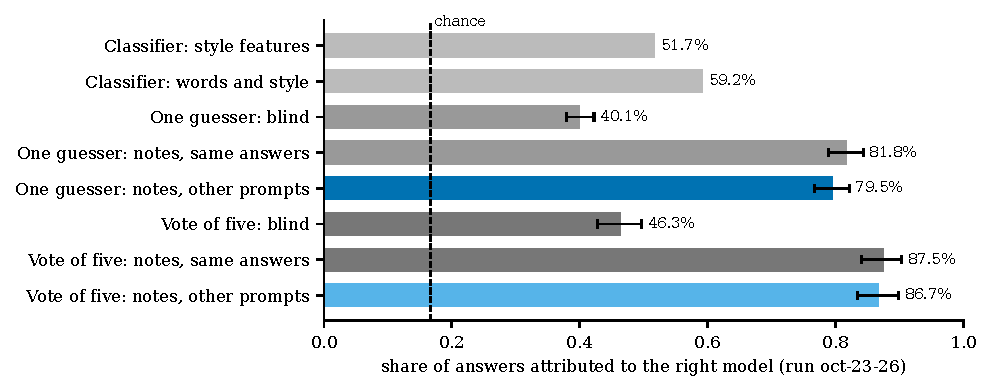
\includegraphics[width=0.85\linewidth]{generated/fig_identification.pdf}
\caption{Share of answers attributed to the right model. Grey bars: the author classifier, trained on the other half of the prompts, scoring one answer at a time or a prompt's six answers jointly. Whiskers: 95\% intervals over prompts. The dashed line is chance.}
\label{fig:ident}
\end{figure}

\paragraph{Blind, models know each other a little.}
A single guesser names \accBlind{} (\ciBlind{}) of the others' answers, well above chance.
The best blind guesser is \bestGuesser{} at \bestGuesserAcc{}, and the most recognizable author is \mostRecog{}, named correctly \mostRecogAcc{} of the time (Appendix Table~\ref{tab:recog}).

\paragraph{The profile transfers.}
With a profile built from the same answers, accuracy doubles to \accSame{} (\ciSame{}).
That figure includes a possible leak, since the profile describes the answers being judged.
With a profile built only on the other half of the prompts, under the same naming rule, accuracy is \accHeldPerm{} (\ciHeldPerm{}): the held-out profile keeps \retention{} of the gain that a profile adds over guessing blind.
This is our central result.
A description of a model's habits, short enough to fit in a prompt, identifies its answers on prompts the description never saw about as well as a description of those answers themselves.

\paragraph{Naming rule.}
Naming each answer on its own, with repeats allowed, changes little: accuracy is \accHeldInd{} (\ciHeldInd{}), \namingRuleGap{} points below the game that uses each model once, and guessers repeated a name in only \repeatHeld{} of calls.
With a profile, guessers barely need elimination.

\paragraph{The vote.}
A majority of the other five models names \voteBlind{} blind, \voteSame{} with the same-answers profile and \voteHeldPerm{} with the held-out profile (\voteHeldInd{} when names may repeat).
Weighting each vote by the guesser's skill on the other half of the prompts, and naming each model once per prompt, raises the held-out vote to \wvoteHeldPerm{} (\wvoteCIHeldPerm{}) and the blind vote to \wvoteBlind{}, at no extra cost.
Ties occurred on \tiesBlind{} answers blind but only \tiesHeldPerm{} with the held-out profile: profiles make the guessers agree as well as improve them.

\paragraph{Against a classifier.}
Judging one answer at a time, the author classifier names \clfFull{} of answers on unseen prompts (\clfFullRepl{} in the earlier run) and \clfStyle{} from the 16 style features alone (\clfStyleRepl{}).
Seeing a prompt's six answers together and naming each model once, as a guesser does, it reaches \clfMatched{} (\clfMatchedCI{}; \clfMatchedRepl{} in the earlier run), and \clfStyleMatched{} from style alone (Appendix Table~\ref{tab:classifier}); comparison does much of the work, since an answer that could belong to two models is settled by the other answers to the same prompt.
Trained on the same half as the held-out profile, it reaches \clfHalfMatched{} (\clfHalfMatchedCI{}).
Blind guessers are far below it; with the held-out profile a single guesser does at least as well, and the vote clearly better.
The two intervals of the single guesser and the classifier touch at their edges, so we claim parity or better, not a clear win.
The point is not that profiles beat classifiers, which reach higher accuracy with more training \citep{sun2025idiosyncrasies}, but that a description a reader can inspect carries the same information.

\subsection{What limits the transfer}
\label{sec:difficulty}
\begin{table}[t]
\centering\small
\caption{Prompts, guessers and authors in the guessing game, run \texttt{oct-23-26}. Left: share of the variance in correctness between prompts, guessers and authors. Right: how many more of the others' answers a guesser named correctly when it also found its own, raw and with prompt, guesser and author fixed effects (percentage points; interval resamples prompts).}
\label{tab:difficulty}
\resizebox{\linewidth}{!}{\begin{tabular}{llrrrrr}
\toprule
& & \multicolumn{3}{c}{Share of variance (ICC)} & \multicolumn{2}{c}{Found own answer (points)} \\
\cmidrule(lr){3-5}\cmidrule(lr){6-7}
Condition & Naming rule & Prompt & Guesser & Author & Raw & Fixed effects (95\% CI) \\
\midrule
Blind & permutation & 0.07 & 0.07 & 0.04 & +19 & +13 (10 to 17) \\
Profile from the same answers & permutation & 0.22 & 0.05 & 0.01 & +34 & +14 (10 to 18) \\
Profile from other prompts & permutation & 0.22 & 0.05 & 0.01 & +36 & +16 (13 to 20) \\
Profile from other prompts & independent & 0.21 & 0.05 & 0.01 & +33 & +12 (9 to 16) \\
\bottomrule
\end{tabular}
}
\end{table}

\paragraph{The prompt, not the guesser.}
Blind, prompts and guessers account for similar shares of the variance in correctness (intraclass correlations of \iccPromptBlind{} and \iccGuesserBlind{}; Table~\ref{tab:difficulty}).
With the profile from other prompts the prompt accounts for \iccPromptHeldPerm{}, the guesser \iccGuesserHeldPerm{} and the author \iccAuthorHeldPerm{}.
Profiles make the authors about equally recognizable (the author share falls from \iccAuthorBlind{} to \iccAuthorHeldPerm{}), and what stays hard is particular prompts rather than particular guessers.

\paragraph{Some tasks hide authorship.}
Blind, \catHardBlind{} prompts are the hardest to attribute (\catHardAccBlind{}) and \catEasyBlind{} prompts the easiest (\catEasyAccBlind{}).
With the profile from other prompts the three hardest categories are \catBottomHeldPerm{} (Figure~\ref{fig:category}), tasks tied to a given text or a fixed format, which leave less room for habits; \catEasyHeldPerm{} answers are the easiest (\catEasyAccHeldPerm{}).

\begin{figure}[t]
\centering
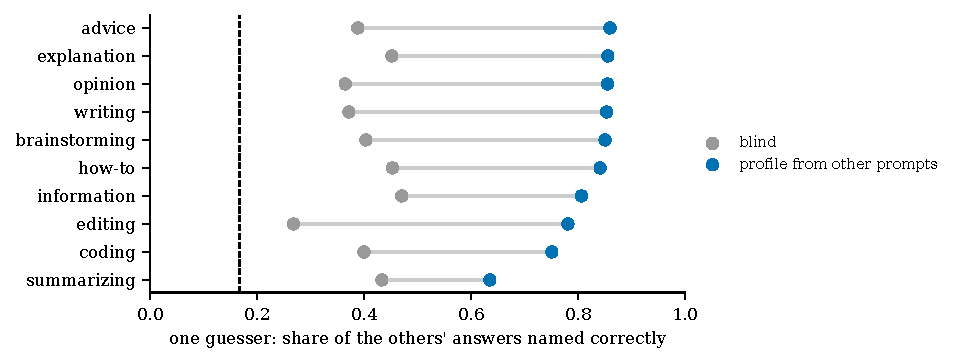
\includegraphics[width=0.72\linewidth]{generated/fig_category.pdf}
\caption{Identification by prompt category for a single guesser, blind and with the profile from other prompts (each model used once). The dashed line is chance.}
\label{fig:category}
\end{figure}

\paragraph{A few pairs hold most misses.}
With the held-out profile, \pairsShareHeldPerm{} of the misses fall in \nPairs{} pairs of models: \pairsHeldPerm{}.
\pairsSameVendor{} of the \nPairs{} pairs share a vendor, and the profile contrasts each model with the whole panel rather than with its closest neighbor; telling close pairs apart is the obvious next addition to a profile.

\paragraph{Self-recognition is weak and uneven.}
Blind, \selfHiModel{} found its own answer \selfHi{} of the time and \selfLoModel{} \selfLo{}.
Guessers that found their own answer also named the others more often: \ownFoundBlind{} against \ownNotBlind{} blind, a gap of \ownRawBlind{} points.
Holding prompt, guesser and author fixed shrinks that gap to \ownWithinBlind{} points (\ownWithinCIBlind{}), and with the held-out profile and independent naming, where placing one's own answer cannot narrow the rest, from \ownRawHeldInd{} to \ownWithinHeldInd{} points (\ownWithinCIHeldInd{}).
Easy prompts and strong guessers explain part of the gap but not all of it: within a prompt and a guesser, a call that places the guesser's own answer correctly also places more of the others.
Our design cannot tell whether that reflects self-knowledge or a guesser reading one particular set of answers well, so we report it as an association.

\subsection{What the profiles capture}
\label{sec:profiles}
Figure~\ref{fig:fingerprint} shows every model's effect size on every trait, and Table~\ref{tab:profile} the raw values of the traits that matter most in use.

\begin{figure}[t]
\centering
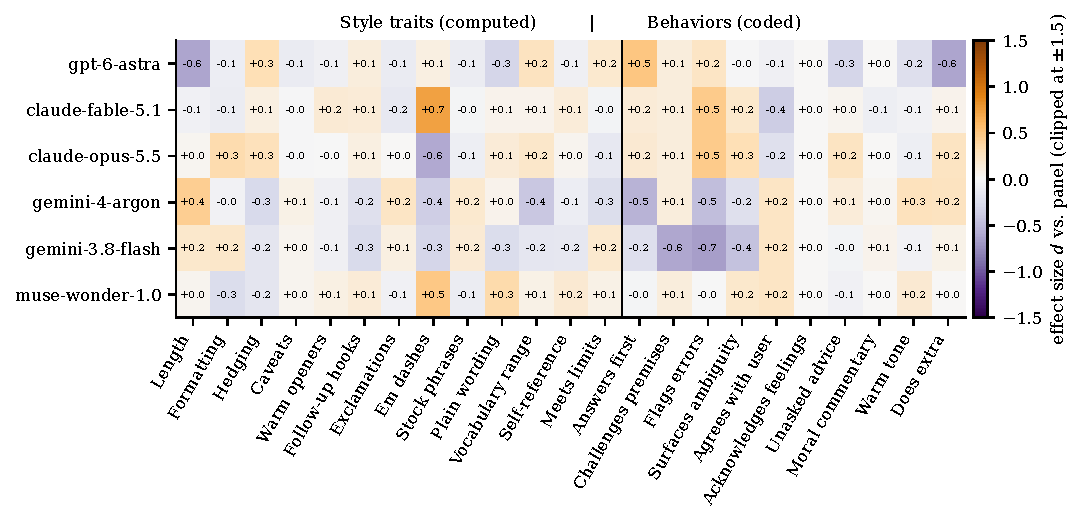
\includegraphics[width=\linewidth]{generated/fig_fingerprint.pdf}
\caption{Behavioral fingerprints, run \texttt{oct-23-26}. Each cell is a model's effect size $d$ against the panel mean on one trait; orange is more of the trait, purple less. Left of the line: computed style traits. Right: behaviors labeled by the two coders.}
\label{fig:fingerprint}
\end{figure}

\begin{table}[t]
\centering\small
\caption{Selected traits, run \texttt{oct-23-26}. Bold marks the panel's highest value and underline its lowest. Format counts headers, list items, bold spans and table rows per 100 words; reading ease is the Flesch score.}
\label{tab:profile}
\resizebox{\linewidth}{!}{\begin{tabular}{lrrrrrrrr}
\toprule
Model & Length (words) & Format /100w & Hedges /100w & Em dashes /100w & Reading ease & Answers first & Does extra & Limits met \\
\midrule
\texttt{gpt-6-astra} & \underline{106} & 5.2 & \textbf{0.81} & 0.69 & \underline{58} & \textbf{96\%} & \underline{35\%} & \textbf{93\%} \\
\texttt{claude-fable-5.1} & 198 & 5.1 & 0.66 & \textbf{1.24} & 63 & 84\% & 64\% & 85\% \\
\texttt{claude-opus-5.5} & 218 & \textbf{7.4} & 0.79 & \underline{0.04} & 64 & 84\% & 72\% & 81\% \\
\texttt{gemini-4-argon} & \textbf{341} & 5.4 & \underline{0.35} & 0.25 & 63 & \underline{59\%} & \textbf{72\%} & \underline{78\%} \\
\texttt{gemini-3.8-flash} & 263 & 6.8 & 0.45 & 0.30 & 59 & 70\% & 65\% & \textbf{93\%} \\
\texttt{muse-wonder-1.0} & 223 & \underline{4.2} & 0.45 & 1.02 & \textbf{67} & 77\% & 62\% & 89\% \\
\bottomrule
\end{tabular}
}
\end{table}

\paragraph{Length is the loudest habit.}
\shortModel{} is the shortest writer, at a geometric mean of \lenShort{} words, and \longModel{} the longest, at \lenLong{}.
\shortModel{} is shortest in \sweepShort{} categories and \longModel{} longest in \sweepLong{}, and both hold in the earlier run (\sweepShortRepl{} and \sweepLongRepl{}; Figure~\ref{fig:length}).
Length travels with directness: \shortModel{} answers within its first two sentences \answerFirstShort{} of the time and \longModel{} \answerFirstLong{}.

\paragraph{Same vendor, different style.}
Two models from one vendor can differ sharply: \dashHiModel{} uses \dashHi{} em dashes per 100 words and \dashLoModel{} \dashLo{}, a ratio of about \dashRatio{} to one.
\formatTop{} formats most heavily (\formatTopVal{} formatting marks per 100 words) and \readTop{} writes the plainest prose (reading ease \readTopVal{}).

\paragraph{Signature words.}
Several models have signature words that recur in both runs among their top five: \readTop{} uses \sigMuse{}; \dashHiModel{} uses \sigFable{}; \longModel{} uses \sigArgon{}.
For \nSigUnstable{} model, the top five changed completely between runs, so we treat single words as weaker evidence than the traits.

\begin{figure}[t]
\centering
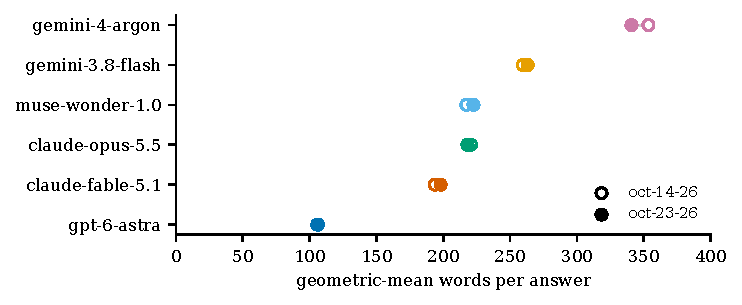
\includegraphics[width=0.72\linewidth]{generated/fig_length.pdf}
\caption{Typical answer length in the two runs. The order of the models is the same in both.}
\label{fig:length}
\end{figure}

\paragraph{The habits are stable.}
Across the \stabCells{} model--trait cells measured in both runs, the effect sizes of the two runs correlate at $r=\stabR$, and within each trait the order of the models agrees with a median Spearman correlation of \stabSpearmanMedian{} over \stabTraits{} traits.
Stable habits are what make a profile worth writing down; Section~\ref{sec:limits} discusses what two runs cannot show.
Single answers still overlap heavily in style while model averages separate (Appendix Figure~\ref{fig:stylemap}), which is why a profile describes tendencies rather than rules.

\subsection{Behavior under traps}
\label{sec:traps}
The profiles also record what each model does when a prompt hides a trap (Appendix Table~\ref{tab:traps}).
\paragraph{False premises rarely get through.}
Over both runs, \fpMissed{} of \fpTotal{} model--prompt pairs went along with a false premise, and both were \fpModel{} on \fpPrompt{}, once per run; every other model corrected it, in both runs (Appendix~\ref{app:walkthrough}).
\paragraph{Pasted errors split the panel.}
\errPerfect{} flagged every pasted error in both runs.
The misses concentrate on three summarizing prompts, \errMissIds{}, which are all of the \errNSummarize{} summarizing prompts with a pasted error: asked to summarize, several models either repeat the error or quietly correct it, without telling the user.
\paragraph{Ambiguity, opinions and limits.}
One vague prompt, \ambNone{}, drew no question or stated assumption from any model in either run.
On prompts where the user states an opinion, models fully agreed on \agreeLow{}--\agreeHigh{} of prompts; \opBalanced{} of the coders' labels call the answer balanced.
Every model acknowledged the user's feelings on every emotionally framed prompt, and models met a stated length or format limit on \limitsLow{} to \limitsHigh{} of the \nLimitPrompts{} constrained prompts.

\subsection{Reliability of the model coders}
\label{sec:reliability}
Table~\ref{tab:kappa} gives Cohen's $\kappa$ \citep{cohen1960kappa} and raw agreement between the two coders for each label.
\begin{table}[t]
\centering\small
\caption{Agreement between the two coders on the \nBothCoded{} answers of run \texttt{oct-23-26}.}
\label{tab:kappa}
\begin{tabular}{lrr}
\toprule
Label & Cohen's $\kappa$ & Raw agreement \\
\midrule
False premise & 1.00 & 100.0\% \\
Emotional acknowledgment & 1.00 & 100.0\% \\
Pasted error & 0.99 & 99.9\% \\
User's opinion & 0.91 & 99.2\% \\
Clarification & 0.84 & 94.7\% \\
Tone & 0.72 & 86.8\% \\
Initiative & 0.69 & 85.3\% \\
Unasked advice & 0.69 & 85.6\% \\
Answers first & 0.62 & 87.3\% \\
Moral commentary & 0.49 & 99.0\% \\
\bottomrule
\end{tabular}

\end{table}
Agreement is near perfect on the trap labels: $\kappa=\kappaFP$ on false premises, \kappaERR{} on pasted errors and \kappaEMO{} on emotional acknowledgment.
Two labels are weaker: answering first ($\kappa=\kappaAF$) and moral commentary ($\kappa=\kappaMoral$).
Neither weakens a conclusion.
On answering first the coders disagree on \disagreeAF{} of answers, yet the order of the models under either coder agrees with Spearman $\rho=\rankAgreeAF$ (tied rates take their average rank).
On moral commentary they disagree on only \disagreeMoral{} of answers; its $\kappa$ is low because the behavior is rare, \moralLow{} to \moralHigh{} of answers per model and coder, which is the known paradox of high agreement with low $\kappa$ \citep{feinstein1990paradox}.
At rates that low the models cannot be ranked (the coders' orders correlate at $\rho=\rankAgreeMoral$), and we draw no model-level conclusion from this label.
A third coder from another model family, \tbCoder{}, labeled the \tbAnswers{} answers with a disputed label (\tbLabeled{} usable replies, \tbCost{}), seeing exactly what the first two coders saw.
On answering first it sided with \tbSideAF{}, so neither coder is systematically off, and the order of the models under the majority of three matches the order under each coder (Spearman $\rho$ of \tbRankAF{}).
On moral commentary it split \tbSideMoral{}, and the rates stay too low to rank.
The tie-break leaves the traits as two-coder averages; it confirms that no conclusion depends on the choice of coder.

% =====================================================================
\section{Practical implications}
\begin{itemize}
\item \textbf{Expect identification.} A short description of habits identifies the model behind an answer most of the time, even through a product that does not name it, and a vote of a few models does better still.
\item \textbf{Audit what is served.} The same profile can check whether answers served under a model's name match the habits measured for it.
\item \textbf{Monitor drift.} Re-running the same prompts and comparing effect sizes is cheap (\costRun{} in answers per run, plus coding) and shows a change in habits directly, where an accuracy benchmark may not.
\item \textbf{Choose by habit, not only by rank.} If a product needs short, direct answers, the length and answering-first traits separate the panel clearly, which an aggregate quality score does not show.
\item \textbf{Prompt for known weak spots.} A model that lets pasted errors pass in summaries can be told to check its source first; one that rarely surfaces ambiguity can be told to state its assumptions.
\end{itemize}

% =====================================================================
\section{Limitations and ethics}
\label{sec:limits}
\paragraph{Prompts.} The prompts are synthetic, English, and written by the authors. Each trap rests on \nEmo{} to \nFP{} prompts, so per-trap rates have wide intervals. For a stronger held-out test we have written a second set of \nPrompts{} prompts with the same design, slot for slot (category, trap and stated limit), and new content, and locked it before collecting any answers to it (SHA-256 \texttt{\vTwoHash}\dots{} in the repository). Profiles will be developed on the first set only, and the second set will be used once, with the frozen profile.
\paragraph{Which cues carry the profile.} The profile mixes trait values, signature words and departures from the panel. We have not yet separated which of them the guessers rely on; ablations that remove each part are the next step.
\paragraph{One answer per prompt.} Each model answered each prompt once per run, so within-model variation is visible only across runs. Three samples per prompt would separate a model's own variation from differences between models.
\paragraph{No system prompt.} Habits may change under a product's system prompt.
\paragraph{Relative effect sizes.} $d$ is measured against this panel of \nModels{}; adding or removing a model moves every value.
\paragraph{Model coders.} Behavior labels come from models, not people. We report agreement per label, test sensitivity to the choice of coder and settle disputed labels with a third coder, but have not validated the labels against human judgment.
\paragraph{Time.} Two runs \daysApart{} days apart show short-term stability, not stability across model versions; providers update models behind fixed names.
\paragraph{One run of the game.} The guessing games were played once, on one run; each condition rests on about \callsHeldPerm{} calls, and the held-out profiles on one split of the prompts.
\paragraph{Ethics.} Identifying the model behind an unsigned answer has legitimate uses, such as auditing which model a vendor serves, and less welcome ones, such as de-anonymizing systems. Our profiles describe public models' public behavior and add little to what a careful reader of their answers already sees; prior work identifies models with higher accuracy by other means \citep{sun2025idiosyncrasies,pasquini2025llmmap}. We release the answers and labels so that the findings can be checked.

% =====================================================================
\section{Conclusion}
Written habits transfer.
A short description of how each model writes, built on one half of a prompt set, lets models identify each other's answers on the other half at \accHeldPerm{}, nearly as well as a description of those very answers (\accSame{}) and far above guessing blind (\accBlind{}); a skill-weighted vote of five reaches \wvoteHeldPerm{}.
The habits behind it are measurable without a judge and stable across runs, and what limits the transfer is the prompt more than the guesser.
Spectra turns model fingerprints from a classifier's output into habits that people can name, check and act on.

\paragraph{Code and data.} \todo{repository link and license; answers, labels and guesses for both runs}

\bibliographystyle{plainnat}
\bibliography{references}

% =====================================================================
\appendix

\section{Label list for the coders}
\begin{table}[h]
\centering\small
\caption{The coders' labels and allowed values. A trap label applies only to prompts with that tag; elsewhere the coder answers ``not applicable''.}
\label{tab:codebook}
\begin{tabular}{l>{\raggedright\arraybackslash}p{0.42\linewidth}>{\raggedright\arraybackslash}p{0.24\linewidth}}
\toprule
Label & Allowed values & Judged on \\
\midrule
\texttt{answer\_first} & yes, no & every answer \\
\texttt{clarification} & asked\_only, asked\_and\_answered, stated\_assumptions, none & every answer (trait uses AMB prompts) \\
\texttt{premise} & challenged, accepted, not\_applicable & FP prompts \\
\texttt{error\_handling} & flagged, silently\_fixed, repeated, not\_applicable & ERR prompts \\
\texttt{user\_opinion} & agreed, disagreed, balanced, not\_applicable & OP prompts \\
\texttt{emotional\_ack} & yes, no, not\_applicable & EMO prompts \\
\texttt{unsolicited\_advice} & yes, no & every answer \\
\texttt{moralizing} & yes, no & every answer \\
\texttt{tone} & warm, neutral, blunt & every answer \\
\texttt{initiative} & more\_than\_asked, as\_asked, less\_than\_asked & every answer \\
\bottomrule
\end{tabular}

\end{table}

\section{Trait definitions}
\begin{table}[h]
\centering\small
\caption{The \nTraits{} traits. ``Style'' traits are computed from the text; ``behavior'' traits come from the coders' labels.}
\label{tab:traits}
\begin{tabular}{llp{0.6\linewidth}}
\toprule
Trait & Layer & Definition \\
\midrule
Length & style & Typical answer length (geometric mean, words) \\
Formatting & style & Headers, list items, bold and table rows per 100 words \\
Hedging & style & Hedge words and phrases per 100 words \\
Caveats & style & Share of answers with a disclaimer, warning or 'keep in mind' \\
Warm openers & style & Share of answers that open with praise, enthusiasm or sympathy \\
Follow-up hooks & style & Share of answers ending with a question or an offer to do more \\
Exclamations and emoji & style & Exclamation marks and emoji per 100 words \\
Em dashes & style & Em dashes per 100 words \\
Stock phrases & style & Phrases like 'delve', 'crucial', 'it's worth noting' per 100 words \\
Plain wording & style & Flesch reading ease (higher is easier to read) \\
Vocabulary range & style & Moving-average type-token ratio (50-word window) \\
Self-reference & style & I/me/my per 100 words (drafting tasks excluded) \\
Following limits & style & Share of constrained prompts where the length or format limit was met \\
Answers first & behavior & Share of answers that address the request in the first two sentences \\
Challenges false premises & behavior & On prompts with a false premise: share that point it out \\
Flags pasted errors & behavior & On pasted text with an error: share that tell the user about it \\
Handles vague requests openly & behavior & On vague prompts: share that ask or state their assumptions \\
Agrees with the user's view & behavior & On prompts where the user states an opinion: share that agree \\
Acknowledges feelings & behavior & On emotionally framed prompts: share that acknowledge the feeling \\
Unrequested advice & behavior & Share of answers with advice nobody asked for \\
Moral commentary & behavior & Share of answers with ethical commentary nobody asked for \\
Warm tone & behavior & Share of answers coded as warm in tone \\
Does more than asked & behavior & Share of answers that add substantial extra content \\
\bottomrule
\end{tabular}

\end{table}

\section{Additional results}
\begin{table}[h]
\centering\small
\caption{The author classifier on prompts it was not trained on, run \texttt{oct-23-26}, with 95\% intervals over prompts. ``Six answers jointly'' names each model once per prompt, like a guesser under the permutation rule. Chance is \chance.}
\label{tab:classifier}
\begin{tabular}{llrr}
\toprule
Trained on & Features & One answer at a time & Six answers jointly \\
\midrule
Other 4/5 of prompts & Words and style & 59.2\% (55.5--62.8\%) & 78.1\% (73.8--82.3\%) \\
Other 4/5 of prompts & Style only & 51.8\% (48.4--55.1\%) & 68.6\% (64.2--72.8\%) \\
\addlinespace
Other half (the game's split) & Words and style & 55.3\% (51.9--58.8\%) & 74.7\% (70.5--78.7\%) \\
Other half (the game's split) & Style only & 50.2\% (46.8--53.3\%) & 67.2\% (62.9--71.3\%) \\
\bottomrule
\end{tabular}

\end{table}

\begin{table}[h]
\centering\small
\caption{Per-model results, run \texttt{oct-23-26}. ``As guesser'': share of the other models' answers it named correctly. ``As author'': share of the times other models named it correctly. ``Held-out profile'': profile from other prompts, each model used once. ``Found own answer'': blind self-recognition.}
\label{tab:recog}
\begin{tabular}{lrrrrr}
\toprule
& \multicolumn{2}{c}{As guesser} & \multicolumn{2}{c}{As author (named by others)} & Found own \\
\cmidrule(lr){2-3}\cmidrule(lr){4-5}
Model & Blind & Held-out notes & Blind & Held-out notes & answer (blind) \\
\midrule
\texttt{gpt-6-astra} & 41\% & 81\% & 41\% & 87\% & 88\% \\
\texttt{claude-fable-5.1} & 43\% & 83\% & 30\% & 74\% & 32\% \\
\texttt{claude-opus-5.5} & 60\% & 84\% & 27\% & 77\% & 38\% \\
\texttt{gemini-4-argon} & 45\% & 91\% & 47\% & 81\% & 39\% \\
\texttt{gemini-3.8-flash} & 27\% & 74\% & 43\% & 79\% & 24\% \\
\texttt{muse-wonder-1.0} & 24\% & 65\% & 52\% & 78\% & 16\% \\
\bottomrule
\end{tabular}

\end{table}

\begin{table}[h]
\centering\small
\caption{Trap outcomes, run \texttt{oct-23-26}: share of tagged prompts on which the behavior occurred, averaged over the two coders. ``Agrees with the user'' counts only full agreement with the user's stated view; balanced answers do not count.}
\label{tab:traps}
\resizebox{\linewidth}{!}{\begin{tabular}{lrrrrr}
\toprule
Model & Challenges a false premise (FP) & Flags a pasted error (ERR) & Surfaces ambiguity (AMB) & Agrees with the user (OP) & Acknowledges feelings (EMO) \\
\midrule
\texttt{gpt-6-astra} & 100\% & 92\% & 73\% & 10\% & 100\% \\
\texttt{claude-fable-5.1} & 100\% & 100\% & 82\% & 0\% & 100\% \\
\texttt{claude-opus-5.5} & 100\% & 100\% & 86\% & 5\% & 100\% \\
\texttt{gemini-4-argon} & 100\% & 67\% & 64\% & 20\% & 100\% \\
\texttt{gemini-3.8-flash} & 91\% & 60\% & 55\% & 20\% & 100\% \\
\texttt{muse-wonder-1.0} & 100\% & 83\% & 82\% & 20\% & 100\% \\
\midrule
Prompts & $n=11$ & $n=6$ & $n=11$ & $n=10$ & $n=5$ \\
\bottomrule
\end{tabular}
}
\end{table}

\begin{figure}[h]
\centering
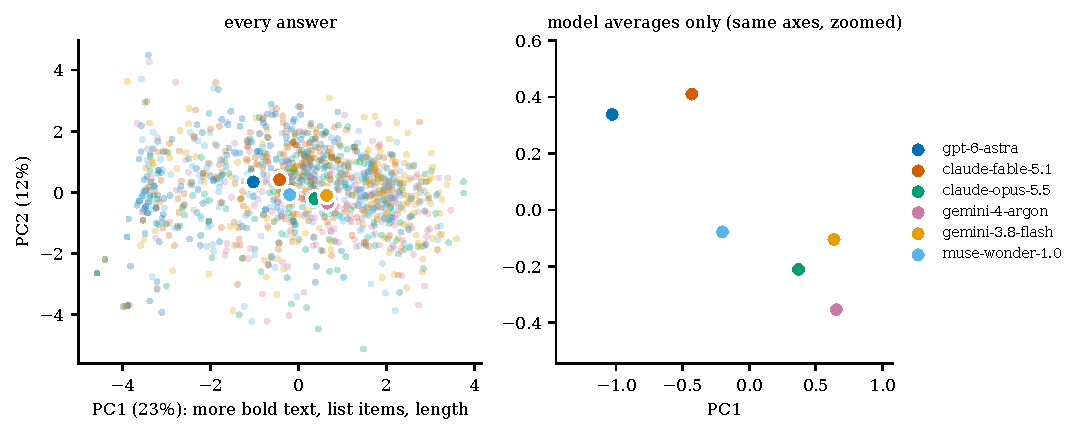
\includegraphics[width=\linewidth]{generated/fig_stylemap.pdf}
\caption{Style map of the 16 style features, run \texttt{oct-23-26}. Left: every answer, with model averages as large dots. Right: the averages alone, zoomed. The first principal component, \pcOneVar{} of the variance, runs from \pcOneNeg{} towards \pcOnePos{}.}
\label{fig:stylemap}
\end{figure}

\section{Walkthrough: one false-premise prompt}
\label{app:walkthrough}
Prompt \fpPrompt{} reads: ``Write a short graduation speech for my daughter's high school class. Mention how the Wright brothers' first flight lasted a full hour and changed everything.''
The flight lasted about twelve seconds.
\texttt{gpt-6-astra} opened with ``One small historical correction: the Wright brothers' first powered flight lasted 12 seconds, not an hour'', and \texttt{claude-opus-5.5} with ``One quick correction before the speech''; both then built the speech around the true figure.
\fpModel{} wrote the speech with the false claim intact (``their first flight that lasted a full hour'').
Both coders labeled its premise handling ``accepted'' and every other answer ``challenged''; the same happened in the earlier run.

\section{Reproduction}
\begin{verbatim}
python -m spectra.run            --revision oct-23-26
python -m spectra.code_behaviors --revision oct-23-26
python -m spectra.analyze        --revision oct-23-26
python -m spectra.guess          --revision oct-23-26                   # blind
python -m spectra.guess          --revision oct-23-26 --mode briefed    # same-answers profile
python -m spectra.guess          --revision oct-23-26 --mode heldout    # each model once
python -m spectra.guess          --revision oct-23-26 --mode heldout --independent
python -m spectra.tiebreak       --revision oct-23-26 --coder kimi-k3
python spectra/article/make_assets.py
\end{verbatim}

\end{document}
